%% using aastex version 6.2
\documentclass[twocolumn, dvipdfmx]{aastex62}
\usepackage{CJK}
\usepackage{textcomp}
\usepackage{graphicx}
\usepackage{here}
\usepackage{hhline}
\usepackage{longtable}

\newcommand\aastex{AAS\TeX}
\newcommand\latex{La\TeX}

\received{\today}
\revised{\today}
\accepted{\today}
\submitjournal{ApJ}

\shortauthors{Goda \& Matsuo}

\begin{document}
\begin{CJK*}{UTF8}{min}

\title{Title}

\author{Shohei Goda}
\affil{\rm Department of Earth and Space Science, Graduate School of Science, Osaka University, 1-1, Machikaneyamacho, Toyonaka, Osaka 560-0043, Japan}

\author{Taro Matsuo}
\affiliation{\rm Department of Earth and Space Science, Graduate School of Science, Osaka University, 1-1, Machikaneyamacho, Toyonaka, Osaka 560-0043, Japan}


\begin{abstract}

Statistically verifying the character of exoplanets, we can expect to reveal the formation or evolution processes of planetary systems. The notable parameters of planetary systems are metallicity of host star, planet mass, and eccentricity. Gas giants around metal rich stars are easily formed by core accretion. Since these planets are grown with bottom up, the distributions of planet masses and eccentricities are seemed to be continuously extended.
On the other hand, the planetary formation by disk instability depends on mass and effective temperature of protoplanetary disk, but there is no strongly dependence on metallicity of host star. As these planets are not formed with bottom up, the planetary masses and eccentricities ununiformly distribute. In this study, we statistically revealed the planetary distributions of metal-rich and -poor regions, and tried to understand the planetary-formation and -evolution processes. Note that we made the dataset included the both selection biases of planetary detection for metal-rich and -poor regions to ignore the effect of these biases. As the results from classification for those samples with Gaussian Mixture Model, we found that the planetary distribution was divided into 3 regions by the boundaries around 3 and 13 $\rm M_J$. We also discovered the different distributions of planet mass between each metallicity region, which explains the different processes of the planetary formation: core accretion model is applied in metal-rich region, and several formation models including core accretion are match in metal-poor region. In addition, we found that the distributions of planetary eccentricity have a difference between each mass cluster, especially in metal-rich region, which implies that there are dynamical interactions after the planets formed by core accretion.


\end{abstract}

\vspace{1cm}

\keywords{methods: data analysis -- planets and satellites: terrestrial planets}


\section{Introduction} \label{sec:introduction}

Decades ago, the discussion of planetary formation in solar system was developed \citep{1985Arizona}, and two formation scenarios for Jupiter was proposed. One of them was core accretion \citep{1974Icar...22..416P, 1980PThPh..64..544M, 1996Icar..124...62P} and the other was disk instability \citep{1951PNAS...37....1K, 1997Sci...276.1836B, 2002Sci...298.1756M}. In theory, the two planetary-formation processes have different dependences on disk metallicity, which is ratio of metal-density-number to hydrogen atoms. For core accretion model, since a protoplanet core needs to grow to the critical core mass, it easily occurs in the metal-rich region promoting the growth \citep{2004ApJ...616..567I, 2012A&A...541A..97M}. Most of planets under 6 $\rm M_J$ are formed by core accretion \citep{2007ApJ...662.1282M}, and under 4 $\rm M_J$ planets have smaller eccentricities than binary stars and more massive planets \citep{2007A&A...464..779R}. The mass distribution of observed gas giants can be also divided into two regions by around 4 $\rm M_J$ \citep{2017A&A...603A..30S}. Because Jupiter's envelope is composed with heavier elements than that of the Sun \citep{2003NewAR..47....1Y}, the core accretion model is widely accepted as the standard formation process for Jupiter. On the other hand, several reports insist whether the planetary formation due to disk instability depends on the metallicity: there exists reports of correlation \citep{2006ApJ...636L.149C, 2007Arizona}, a very weak positive correlation \citep{2007ApJ...661L..77M}, and no correlation \citep{2002ApJ...567L.149B} between disk metallicity and disk instability in the metallicity range of the stars hosting the observed planets. 

Since the first planet around a normal star was discovered in 1995
\citep{1995Natur.378..355M}, by the large-sized radial velocity observations, it was revealed that gas giants in the extrasolar system often exist around metal-rich stars \citep{2003A&A...398..363S, 2005ApJ...622.1102F}, and that the amount of metallicity in a planetary system having small planets is less than having gas giants \citep{2011arXiv1109.2497M, 2015AJ....149...14W}. It seems that almost all gas giants are formed via core accretion because the central star and its surrounding protoplanetary disk are composed with the same molecular cloud \citep{2004ApJ...616..567I, 2012A&A...541A..97M}. Since the radial velocity observation can detect the planetary masses or orbital eccentricities with good accuracy, we focus the dataset observed by radial velocity.

The planetary-formation theories showed above are based on the observed data, whose distributions are assumed to be close to real model. However, some data was obtained with poor accuracy or short time of observation, which include biases depended on the metallicity. Because these poor observations restrict the detection possibility for planets, the distribution of discovered planets possibly include some underpopulated regions due to the selection biases. Furthermore, the previous studies insist that under 4 $\rm M_J$ planets are formed by core accretion, and over 4 $\rm M_J$ planets are explained by disk instability, but it is possible to form the massive planets under 30 $\rm M_J$ through core accretion in theory \citep[e.g.,][]{2009A&A...501.1161M, 2016ApJ...823...48T}

In this paper, we discuss the two planetary-formation processes for the planetary distribution discovered by the radial velocity with considering the selection biases. We explain how the samples used in this study are selected and how to use the data considered the selection bias in Section \ref{sec:method}. We also classify the planetary distribution in different region of metallicity, and check the distributions of planetary mass and eccentricity in each region and cluster in Section \ref{sec:results}. Finally, we discuss the planetary-formation and -evolution processes from the results.


\section{Method} \label{sec:method}

In this section, we explain how the planet samples used for this study are collected and restricted, and how we compare the effects of selection bias with different regions of metallicity.


\subsection{Preparing Data} \label{subsec:prepare}

The samples considered in this paper are limited to companion objects detected by radial velocity observations, allowing the orbital parameters to be characterized and the lower limit of the companion mass to be determined. Essentially, samples are selected from those labeled “Radial Velocity” in the “detection method” column of the Extrasolar Planet Encyclopedia catalog53 as of the end of June 2018 \citep{2011A&A...532A..79S}. The radial velocities of central stars by orbiting planets, the orbital periods, and eccentricities of planets are also collected from same catalog. On the other hand, the masses and metallicities of host stars are cited from the SWEET-Cat catalog \citep{2018A&A...620A..58S}, and the lower limit of companion masses are calculated with an equation showed in \cite{2008ApJ...677.1324T}. The radii of planets are calculated from the orbital periods and star masses. The data is also extracted from the Casagrande catalog \citep{2011A&A...530A.138C}, the Padova database \citep{2000A&AS..141..371G}, and the BaSTI stellar model \citep{2018ApJ...856..125H}. Then, the correlation between the data from the SWEET-Cat catalog and the others is checked in order to fill up the data lacking of host stars' masses or metallicities with linear conversion. In addition, the accuracy and terms of observations for each planetary system as indicators of selection biases are extracted from exoplanets.org. The observation terms and star masses supply the upper limit of semi-major axes for the planetary systems. The semi-major axes of planets, the star masses, and the accuracy of observations are used for calculation of observable lower limit of planet masses. The other lacking data is filled up with several studies (この文章は必要か?).

The gaseous objects from all the samples used in this study are extracted in order to remove the impact of low-mass samples, such as Neptune-mass planets (gas dwarfs) and super-Earths. First, we determined the boundary mass between the gaseous and gas-dwarf objects from a perspective of both theory and observation. According to a previous study \citep{2004ApJ...604..388I}, gas-dwarf objects, which primarily consist of heavy-core objects such as Neptune and Uranus, have the potential to grow to the extent allowed by the core building materials inside their semi-major axes. This growth occurs via giant impacts in the inner region of the disk after the disk gas dissipates. However, this core growth is limited by the scattering effect of the heavy core increasing with greater distances from the central star. Therefore, the mass of a gas-dwarf object reaches a maximum at the semi-major axis, where the scattering effect begins to limit the core growth. Given that the ratio of the collision-to-ejection probabilities for the heavy core is 0.1 and the core density is 1 $\rm g/cm^3$, the upper limit on the mass of a gas-dwarf object is about 0.37 $\rm M_J$. Considering a factor of the solid-angle average, the upper mass limits on a gas-dwarf object are estimated to be approximately 0.1 and 0.3 $\rm M_J$. On the other hand, a boundary between gas giants and gas dwarfs at four times the Earth's radius has been observationally revealed by the Kepler data \citep{2012Natur.486..375B}. From the empirical planetary mass-radius relation \cite{2013ApJ...768...14W}, we found that the boundary of planetary mass is less than 150 times the Earth's mass and consistent with the above theoretical estimation. Based on these considerations, 0.1 $M_J$ is applied in this study as the boundary mass between gas giants and gas dwarfs. Performing these preprocessing for all data observed by radial velocity observations, we use 520 planetary systems and 623 planets in this study.


\subsection{Selection Bias} \label{subsec:bias}

When a planetary system is observed, the upper limit of semi-major axis, $a|_{max}$, and lower limit of planet mass, $M_p\sin i|_{min}$, in the system can be estimated with the accuracy of observation, $\sigma$, and observational term, $\tau$ as below \citep{2008ApJ...677.1324T},
\begin{eqnarray}
a|_{max} &=& M_{*}^{\frac{1}{3}}\tau^{\frac{2}{3}} , \\
M_p\sin i|_{min} &=& 4.919\times10^{-3}P^{\frac{1}{3}}(1-e^2)^{\frac{1}{2}}M_{*}^{\frac{2}{3}}\sigma ,
\end{eqnarray}
where, $M_*$, $P$, and $e$ are the star mass, orbital period, and eccentricity of planet, respectively. Each signal coming from the objects include selection biases as above, which have different effects depending on the metallicities of the systems (Figure \ref{fig:bias}, (a)). Therefore, the planets in the different region of metallicity have potentially selection biases, and this effect should be considered for discussing the planetary distribution. Now, we made the non-bias data that was filtered with the selection biases of the opposite region of metallicity in order to remove the bias effect (Figure \ref{fig:bias}, (b)). We show how the difference of selection bias affects the planetary distribution from verifying the two regions in Section \ref{sec:results}.


\begin{figure}[t]
\begin{center}
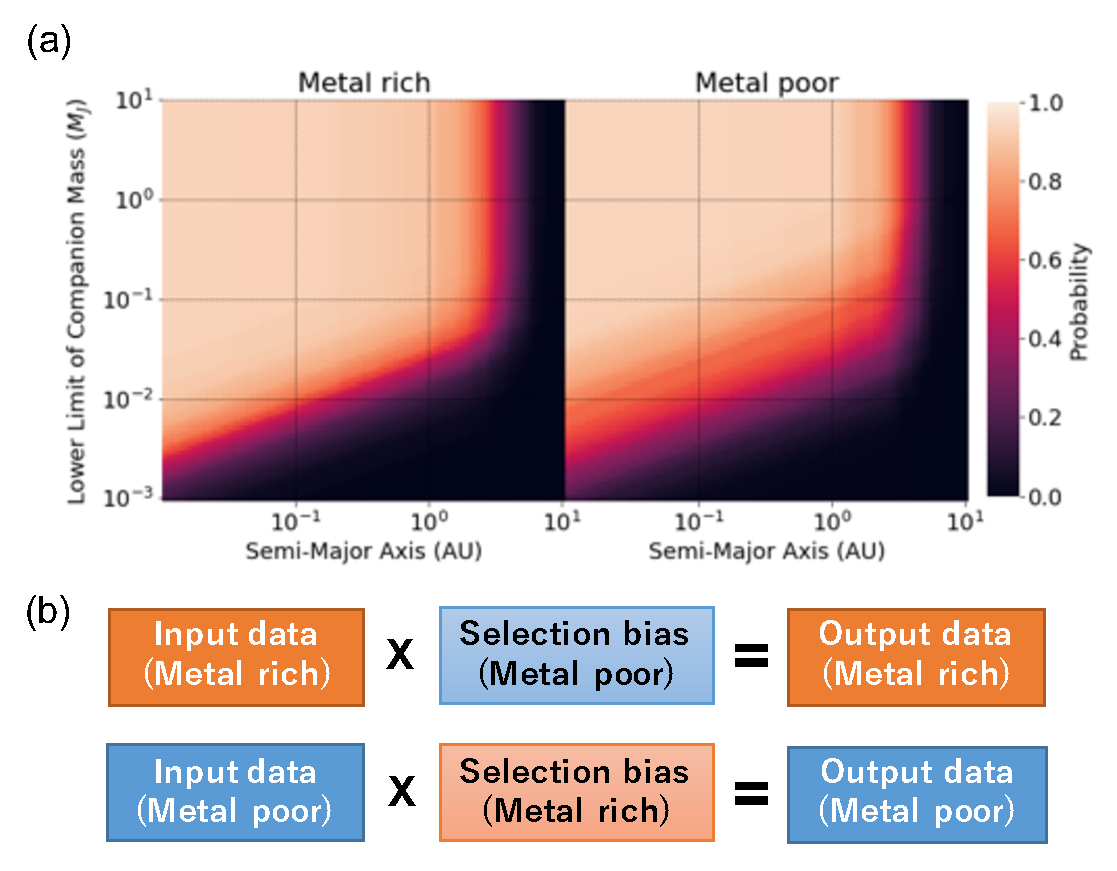
\includegraphics[width=9cm]{../../../Figure/selection_bias.pdf}
\caption{(a) The detectable regions for metal-rich systems (left) and metal-poor systems (right). The boundary of metallicity is fixed as 0.0 dex. Each planetary system is observed with the detection probability. (b) The method of making dataset. Each data is filtered with the opposite selection bias for flatting the differences between detection ranges. \label{fig:bias}}
\end{center}
\end{figure}


\section{Results} \label{sec:results}

In this section, we quantitively show how the selection biases in the different metal regions affects, and classify the planetary distributions into several clusters with Gaussian Mixture Model (GMM). We also discuss the differences of planetary-mass distributions and eccentricity distributions between the classified clusters.


\subsection{Planetary-Mass Distribution} \label{subsec:mass}

First, we determined the boundary of metallicity, which makes the two divided planetary-mass distributions as most different, to verify the possibility of the effect due to the selection biases, and compared the two regions. Changing the metallicity boundary from -0.7 to 0.4 dex, we made the two regions' dataset, and evaluated the planetary-mass distributions with Anderson-Darling (AD) test. Note that we extracted randomly the values of planetary parameters considered their errors, and filtered each sample with any selection biases to remove the calculation bias. Then, the simulations were iterated until the value of boundary was settled. As the result, we found that the best border of metallicity is -0.09 dex. Dividing data with this border, we compared the planetary-mass distributions of both regions. The left of Figure \ref{fig:a_Mp}, (a) shows the relation between semi-major axes and planetary mass, and the right one is the cumulative of planetary mass. AD test for the metal-rich and -poor regions showed that the p-value is $5.6\times10^{-5}$, which can low enough to dismiss the two samples. Thus, we proposed that there is no effect of selection biases for planetary distribution, and exists a difference between the each metallicity region.

Second, we divided the planet samples into two regions with the optimized boundary of metallicity, and classified each planetary distribution with a classifier. In this study, we used GMM, which can classify the samples as the number of clusters assumed that each sample extend as a gaussian distribution \citep[e.g.,][]{2012MNRAS.424.2832L}. Converting the number of clusters, we evaluated each model with Bayesian Information Criterion (BIC), and found the best number of clusters for these samples. Then, both the samples in a metal-rich and -poor regions were optimized as the numbers of clusters were three, when the scores of BIC were 2644 and 1197, respectively.  Figure \ref{fig:a_Mp}, (b) shows the result of classification of planetary distribution with the best number of clusters. The black dash lines are the borders of planetary masses dividing the samples into three regions. These boundaries were drawn at 2.8 and 11.5 $\rm M_J$ in a metal-rich region, and 3.5 and 20.0 $\rm M_J$ in a metal-poor region, respectively.

\begin{figure}[t]
\begin{center}
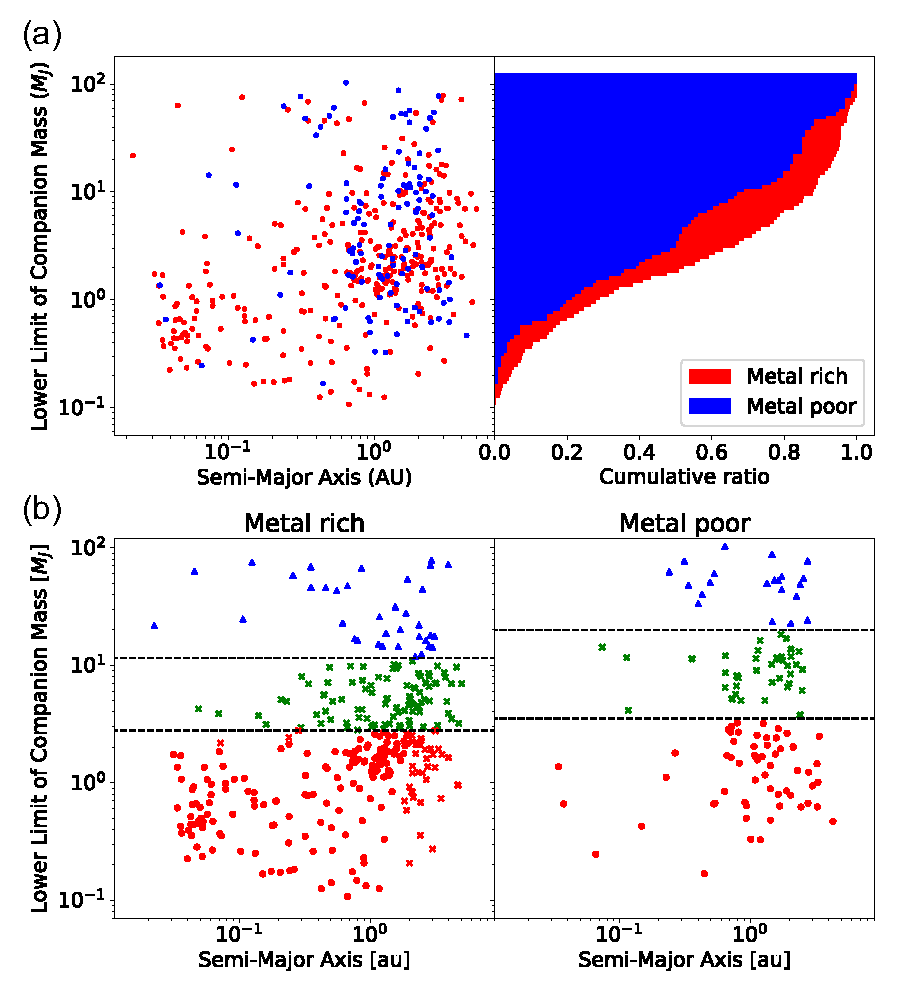
\includegraphics[width=9cm]{../../../Figure/a_Mp.pdf}
\caption{(a) The left is planetary distribution divided by the optimized boundary of metallicity. The red and blue points are the metal-rich and -poor samples, respectively. The right is the cumulative maps of the planetary masses in each region. (b) The result for classification of planetary distributions in each metal range with GMM. The marks in this figure are corresponding to each cluster label. The red, green, and blue points are used as the low-, middle-, and high-mass fields of planets. The black dash lines show the boundaries of planetary mass. \label{fig:a_Mp}}
\end{center}
\end{figure}


\subsection{Eccentricity Distribution} \label{subsec:eccentricity}

The tops of Figure \ref{fig:e_Mp} are scatter maps of eccentricities and lower limit of companion masses in each metal region after classification of planetary distribution with the mass boundaries obtained from GMM. The bottoms are the cumulative maps of the eccentricities in each region and cluster. In the metal-poor region, the distribution of high-mass field is more uniform than any other field. When the samples of high-mass field were compared with those of low- or middle-mass fields by AD test, the p-values were $2.3\times10^{-3}$ and $1.1\times10^{-2}$, respectively. This result is consistent with previous studies (参考文献). In contrast, the middle- and high-mass fields are extending as uniform in the metal-rich region. We also evaluated the samples of low-mass field to those of middle- or high-mass fields by AD test, and found that the p-values were $1.6\times10^{-5}$ and $4.4\times10^{-4}$, respectively. This result implies the possibility that the middle-mass planets were excited by something interaction and their eccentricities
grew.

\begin{figure}[t]
\begin{center}
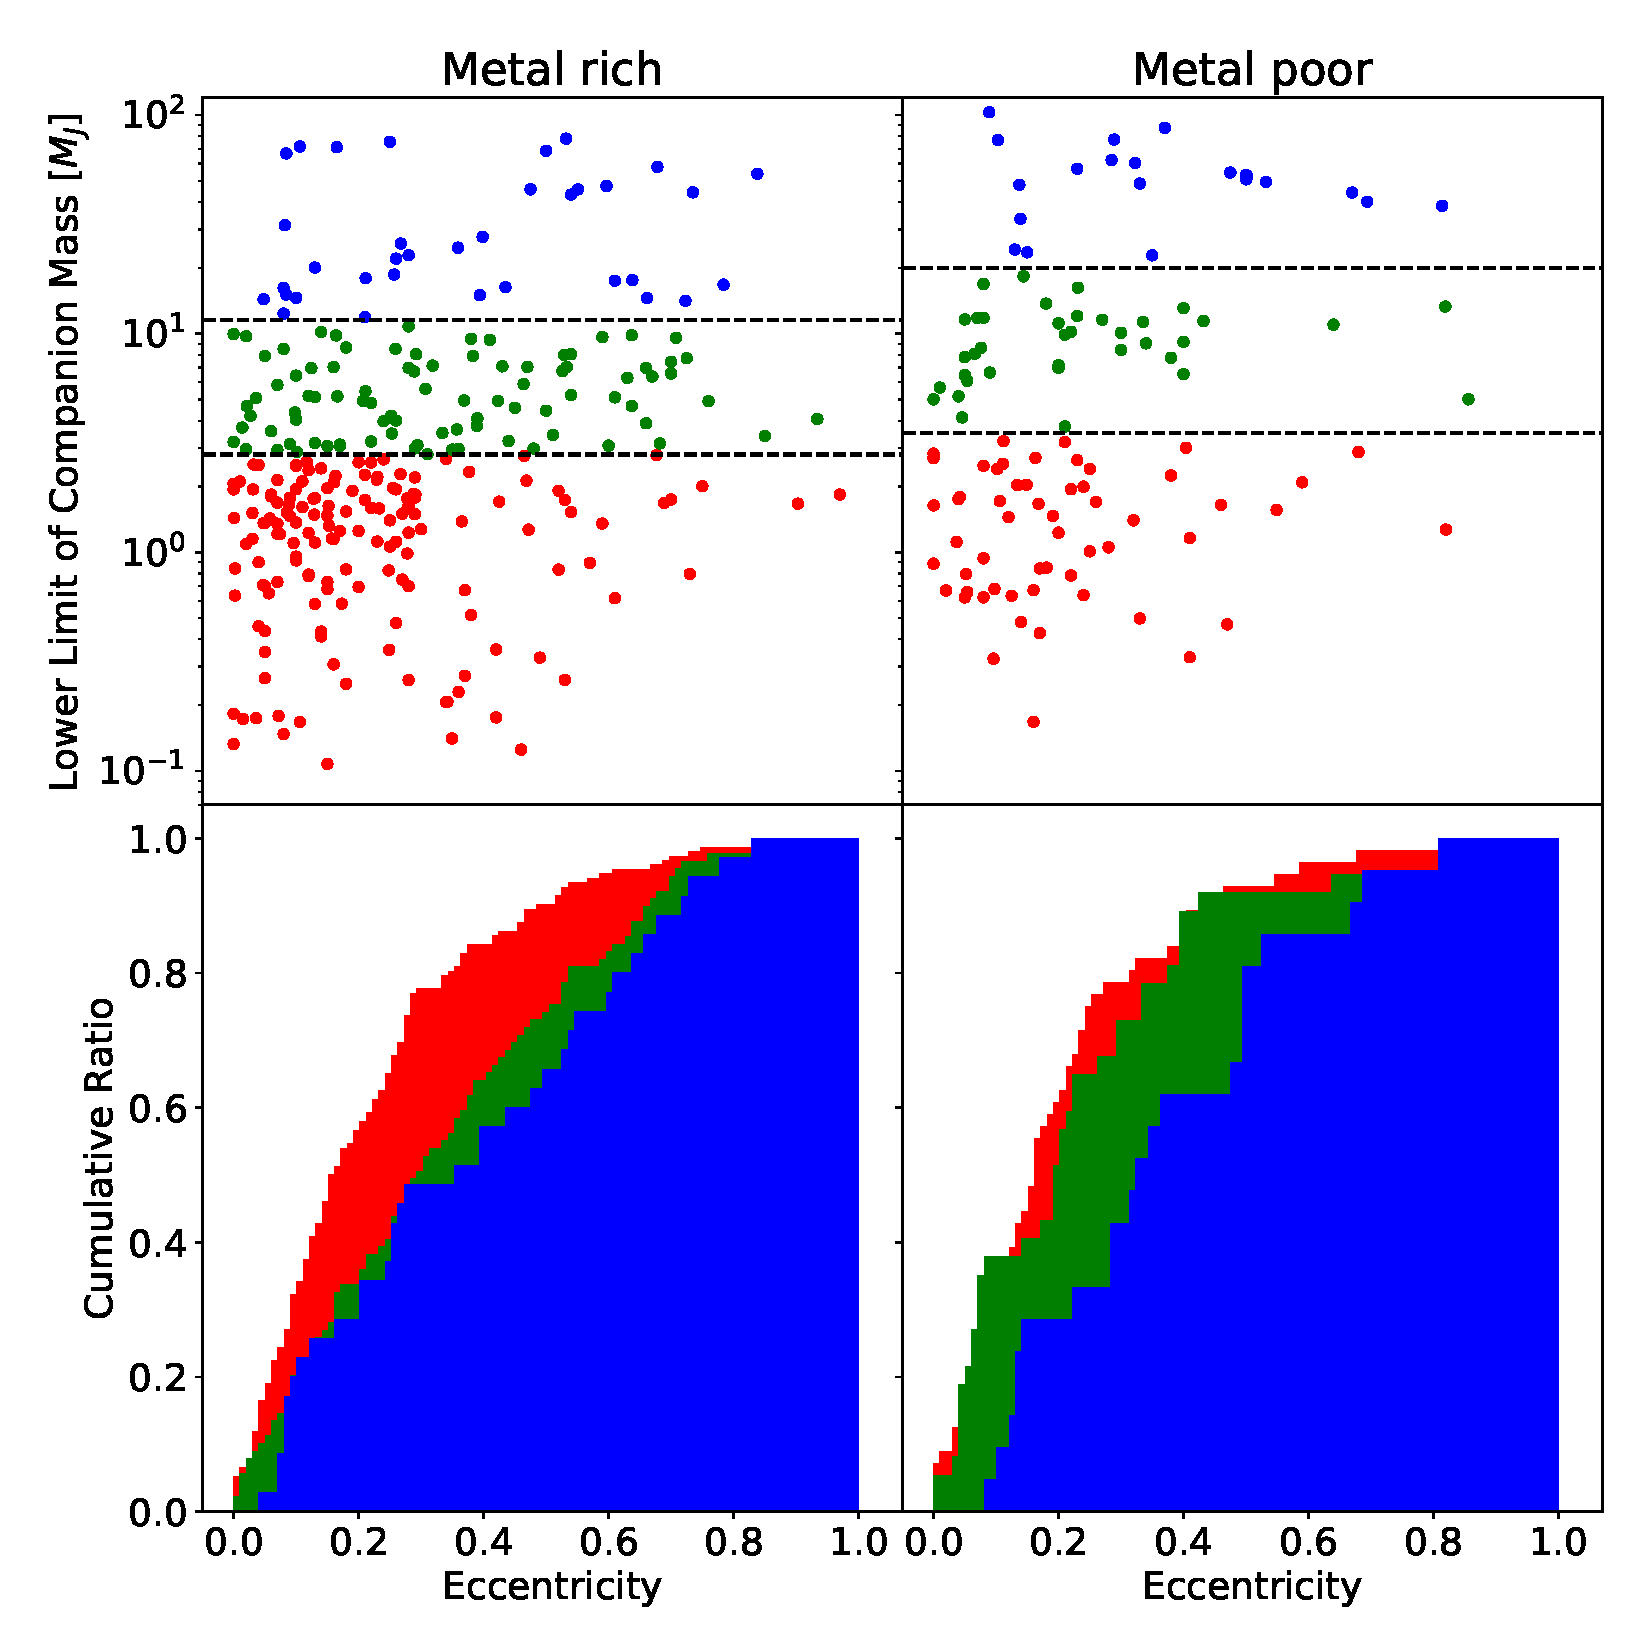
\includegraphics[width=9cm]{../../../Figure/e_Mp_merge.pdf}
\caption{Scatter maps of eccentricities and lower limit of companion masses (top), and cumulative maps of eccentricities (bottom). These colors are the same as those of Figure \ref{fig:a_Mp}, (b), and corresponding to the top and bottom figures. \label{fig:e_Mp}}
\end{center}
\end{figure}


\section{Discussion}

In this section, we compare the above results of planetary mass and eccentricity distributions with previous studies and verify the relationship. We also discuss the behavior of planetary distributions in the metal-rich and -poor regions, comparing the observed dataset from the simulation of \cite{2012A&A...541A..97M}.


\subsection{Relationship with Previous Studies}

First, we discuss the planetary mass distribution. According to previous studies, the distribution of gas-giant masses can be divided into two regions by the border of 4 $\rm M_J$ with metallicity bias, which insists that the planetary-formation processes in each region are different \citep[e.g.,][]{2017A&A...603A..30S}. In contrast, the boundaries were drawn at about 3 and 13 $\rm M_J$ from our result, which the former is almost consistent with the previous studies. The latter indicates the border between the gas giants and brawn dwarfs.

Second, we discuss the distribution of eccentricities. The interaction between a gas giant and protoplanetary disk possibly makes the eccentricity of planet grow \citep{2003ApJ...585.1024G, 2006A&A...447..369K}. This interaction is concentrated at discrete Lindblad and corotation resonances, which causes the planet's orbit to migrate and open a gap in the disk as the planet mass is large enough. If the viscous coefficient equals to $10^{-5}$, the planet with circular orbit changes to eccentric orbit as the planetary mass is over 3 $\rm M_J$. The more massive planets make their eccentricity higher by the maximum value 0.25. On the other hand, if a planetary system has two gas giants, the outer planet may prolong the orbital period of the inner planet. These planets' eccentricities grow up in rough inverse proportion to their masses by this orbital interaction \citep{2002ApJ...564L.105C}. From the verification of simulation \citep{2013ApJ...775...42I}, gas giants and rocky/icy planets emerge, migrate, and undergo dynamical instability in a relatively massive disk, and the perturbation between planets causes orbital crossing, eccentricity excitation, and planetary ejection. The eccentricity of gas giants formed via disk instability ranges from 0 to 0.35 in initial stage \citep{2011ApJ...731...74B}. Then, the range of semi-major axis is $30\sim70$ au. Against above reports, we verified the eccentricity distributions in both metal-rich and -poor regions, where the planetary masses are divided into three fields. As the result, the distributions of middle-mass planets in the metal-rich and -poor regions have obvious difference. In the metal-poor region, the distribution of middle-mass planets is similar to that of low-mass planets, and extends continuously. In contrast, the middle-mass planets distribute differently from low-mass planets, but uniformly such as the massive planets' field. This is because a dynamical interaction occurred in a disk after planetary formation, which leads the eccentricity of planet to grow.


\subsection{Confirmation the Planetary-Formation Process}

In \cite{2012A&A...541A..97M}, planets are formed by classical core accretion model, and the final semi-major axes and planetary masses are determined, based on the simulation included the planetary migration in disks and the disk evolution. From our study, the two observed planetary-mass distributions, which were divided by the metal boundary, had different expanses. Then, we discuss each planetary-formation process, comparing the distribution of observed data with that of simulation data. Figure \ref{fig:discussion} shows that the comparison between the observed data included the selection biases and simulation data cited from \cite{2012A&A...541A..97M}. The simulation data were also filtered by both selection biases of metal-rich and -poor regions to complete the conditions with the observed data. As the result, the distributions of metal rich regions are very consistence, which can explain that most of gas giants in the metal rich region are formed by core accretion. (metal poorについては?)

\begin{figure}[b]
\begin{center}
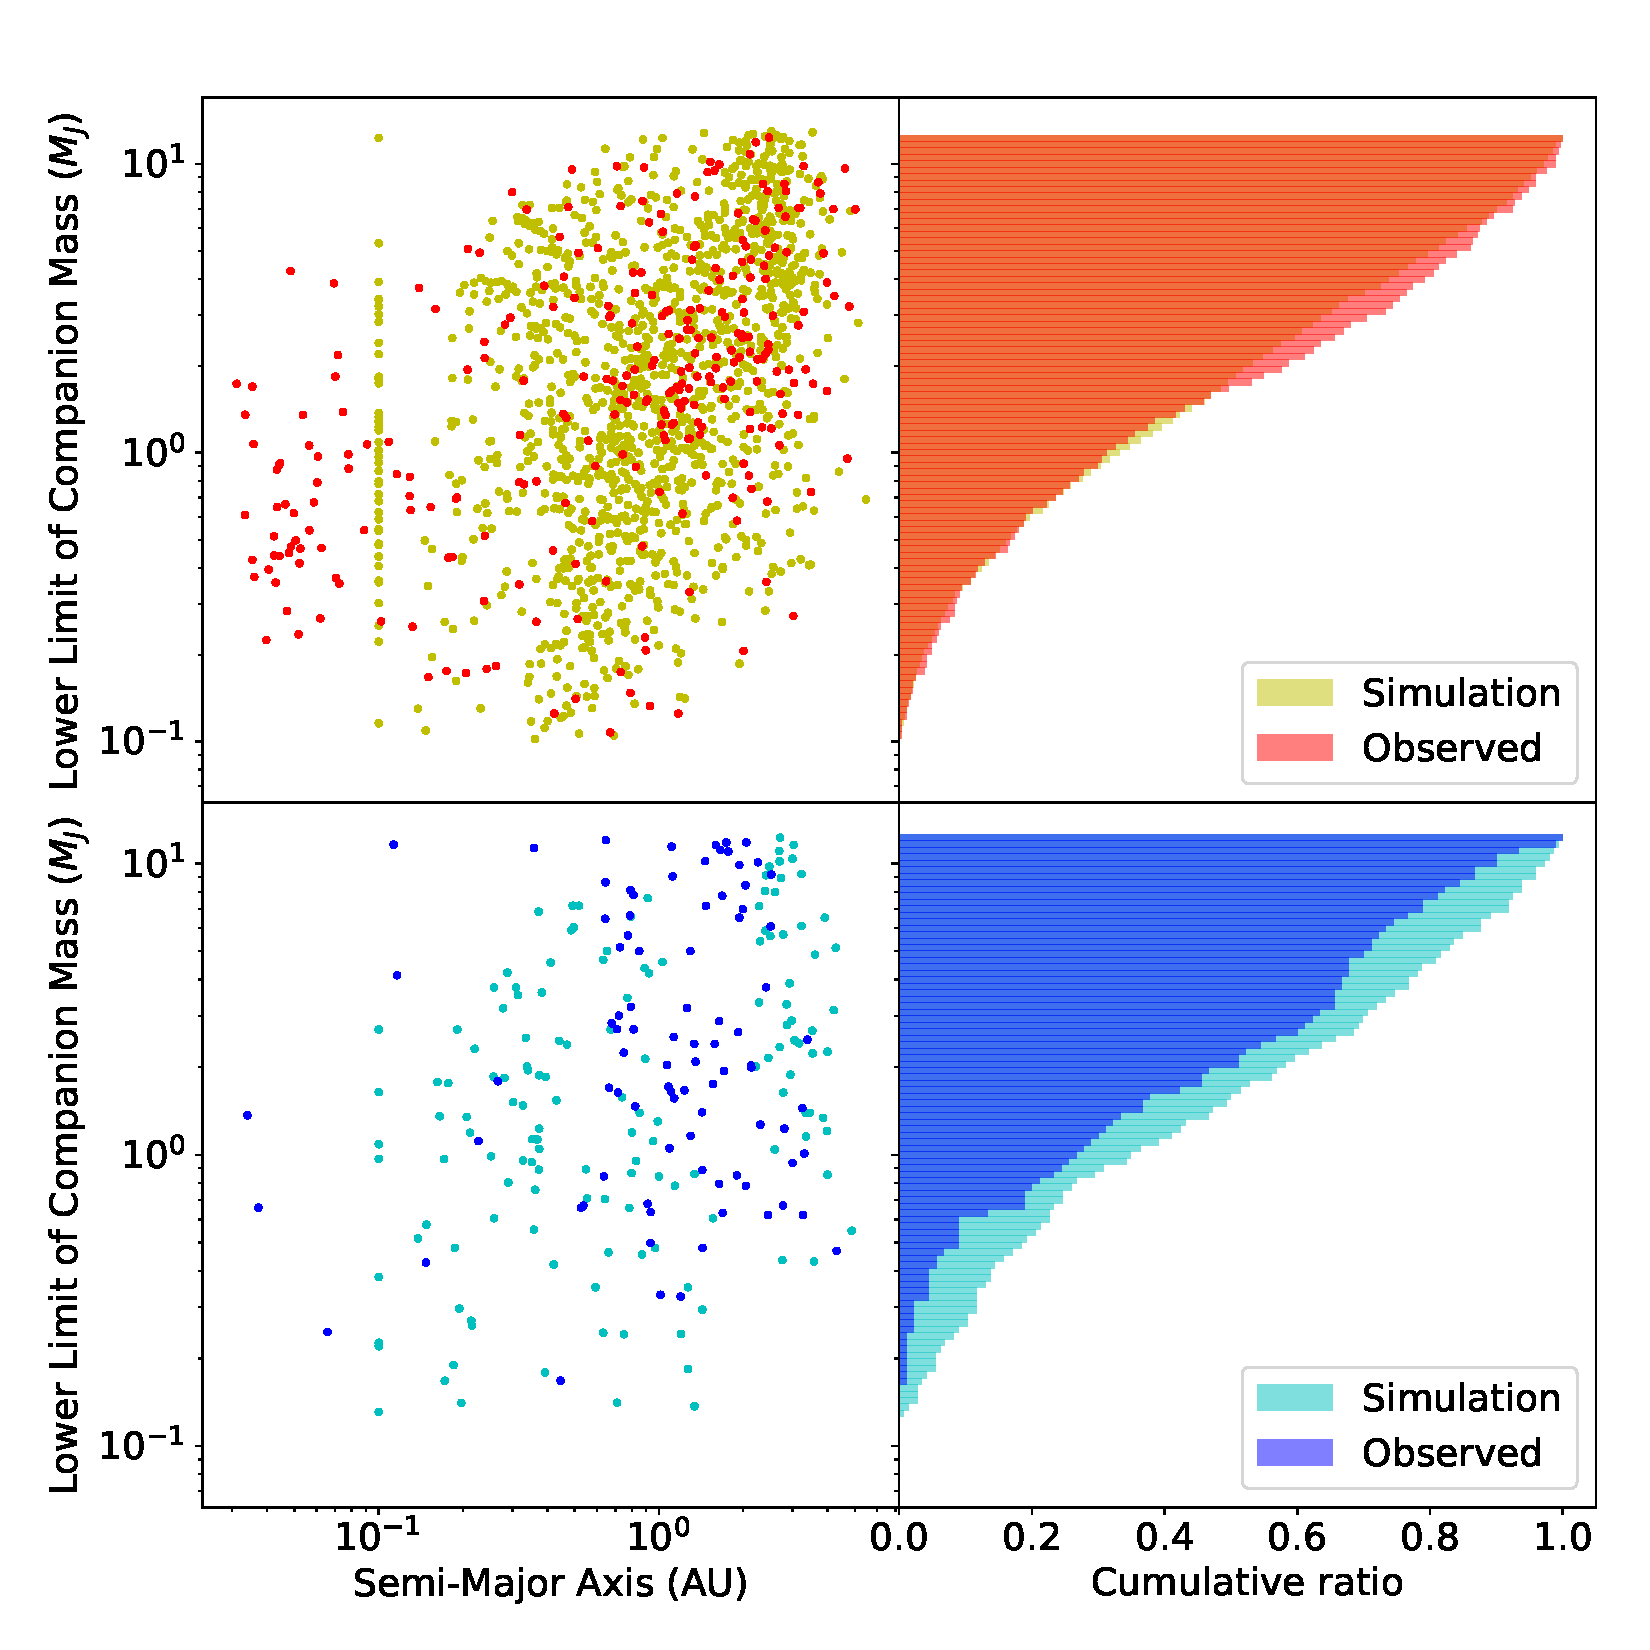
\includegraphics[width=9cm]{../../../Figure/discussion.pdf}
\caption{Comparison of planetary distributions between the observed data (red and blue points) and simulation data (yellow and cyan points) in the metal-rich region (upper left) and the metal-poor region (lower left), and the cumulative maps of planetary masses in the metal-rich region (upper right) and the metal-poor region (lower right). \label{fig:discussion}}
\end{center}
\end{figure}


\acknowledgments


\vspace{5mm}


\begin{thebibliography}{}

\bibitem[Boss(1997)]{1997Sci...276.1836B} Boss, A.~P.\ 1997, Science, 276, 1836
\bibitem[Boss(2002)]{2002ApJ...567L.149B} Boss, A.~P.\ 2002, \apjl, 567, L149
\bibitem[Boss(2011)]{2011ApJ...731...74B} Boss, A.~P.\ 2011, \apj, 731, 74
\bibitem[Buchhave et al.(2012)]{2012Natur.486..375B} Buchhave, L.~A., Latham, D.~W., Johansen, A., et al.\ 2012, \nat, 486, 375
\bibitem[Cai et al.(2006)]{2006ApJ...636L.149C} Cai, K., Durisen, R.~H., Michael, S., et al.\ 2006, \apjl, 636, L149
\bibitem[Casagrande et al.(2011)]{2011A&A...530A.138C} Casagrande, L., Sch{\"o}nrich, R., Asplund, M., et al.\ 2011, \aap, 530, A138
\bibitem[Chiang et al.(2002)]{2002ApJ...564L.105C} Chiang, E.~I., Fischer, D., \& Thommes, E.\ 2002, \apjl, 564, L105
\bibitem[Durisen et al.(2007)]{2007Arizona} Durisen, R. H., Reipurth, V. Jewitt, Keil, K., et al.\ 2007, Univ. of Arizona Press, Tucson 951, 607-622
\bibitem[Fischer \& Valenti(2005)]{2005ApJ...622.1102F} Fischer, D.~A., \& Valenti, J.\ 2005, \apj, 622, 1102
\bibitem[Girardi et al.(2000)]{2000A&AS..141..371G} Girardi, L., Bressan, A., Bertelli, G., \& Chiosi, C.\ 2000, \aaps, 141, 371
\bibitem[Goldreich \& Sari(2003)]{2003ApJ...585.1024G} Goldreich, P., \& Sari, R.\ 2003, \apj, 585, 1024
\bibitem[Hayashi\&Nakagawa(1985)]{1985Arizona} Hayahi, C., Nakazawa, K., \& Nakagawa, Y.\ 1985, Formation of the solar system. Protostars and Planets II. Tucson AZ, University of Arizona Press 1100-1153
\bibitem[Hidalgo et al.(2018)]{2018ApJ...856..125H} Hidalgo, S.~L., Pietrinferni, A., Cassisi, S., et al.\ 2018, \apj, 856, 125
\bibitem[Ida \& Lin(2004)]{2004ApJ...604..388I} Ida, S., \& Lin, D.~N.~C.\ 2004, \apj, 604, 388
\bibitem[Ida \& Lin(2004)]{2004ApJ...616..567I} Ida, S., \& Lin, D.~N.~C.\ 2004, \apj, 616, 567
\bibitem[Ida et al.(2013)]{2013ApJ...775...42I} Ida, S., Lin, D.~N.~C., \& Nagasawa, M.\ 2013, \apj, 775, 42
\bibitem[Kley \& Dirksen(2006)]{2006A&A...447..369K} Kley, W., \& Dirksen, G.\ 2006, \aap, 447, 369
\bibitem[Kuiper(1951)]{1951PNAS...37....1K} Kuiper, G.~P.\ 1951, Proceedings of the National Academy of Science, 37, 1
\bibitem[Lee et al.(2012)]{2012MNRAS.424.2832L} Lee, K.~J., Guillemot, L., Yue, Y.~L., Kramer, M., \& Champion, D.~J.\ 2012, \mnras, 424, 2832
\bibitem[Matsuo et al.(2007)]{2007ApJ...662.1282M} Matsuo, T., Shibai, H., Ootsubo, T., \& Tamura, M.\ 2007, \apj, 662, 1282
\bibitem[Mayor \& Queloz(1995)]{1995Natur.378..355M} Mayor, M., \& Queloz, D.\ 1995, \nat, 378, 355
\bibitem[Mayer et al.(2002)]{2002Sci...298.1756M} Mayer, L., Quinn, T., Wadsley, J., \& Stadel, J.\ 2002, Science, 298, 1756
\bibitem[Mayer et al.(2007)]{2007ApJ...661L..77M} Mayer, L., Lufkin, G., Quinn, T., \& Wadsley, J.\ 2007, \apjl, 661, L77
\bibitem[Mayor et al.(2011)]{2011arXiv1109.2497M} Mayor, M., Marmier, M., Lovis, C., et al.\ 2011, arXiv:1109.2497
\bibitem[Mizuno(1980)]{1980PThPh..64..544M} Mizuno, H.\ 1980, Progress of Theoretical Physics, 64, 544
\bibitem[Mordasini et al.(2009)]{2009A&A...501.1161M} Mordasini, C., Alibert, Y., Benz, W., \& Naef, D.\ 2009, \aap, 501, 1161
\bibitem[Mordasini et al.(2012)]{2012A&A...541A..97M} Mordasini, C., Alibert, Y., Benz, W., Klahr, H., \& Henning, T.\ 2012, \aap, 541, A97
\bibitem[Perri \& Cameron(1974)]{1974Icar...22..416P} Perri, F., \& Cameron, A.~G.~W.\ 1974, \icarus, 22, 416
\bibitem[Pollack et al.(1996)]{1996Icar..124...62P} Pollack, J.~B., Hubickyj, O., Bodenheimer, P., et al.\ 1996, \icarus, 124, 62
\bibitem[Ribas \& Miralda-Escud{\'e}(2007)]{2007A&A...464..779R} Ribas, I., \& Miralda-Escud{\'e}, J.\ 2007, \aap, 464, 779
\bibitem[Santos et al.(2003)]{2003A&A...398..363S} Santos, N.~C., Israelian, G., Mayor, M., Rebolo, R., \& Udry, S.\ 2003, \aap, 398, 363
\bibitem[Santos et al.(2017)]{2017A&A...603A..30S} Santos, N.~C., Adibekyan, V., Figueira, P., et al.\ 2017, \aap, 603, A30
\bibitem[Schneider et al.(2011)]{2011A&A...532A..79S} Schneider, J., Dedieu, C., Le Sidaner, P., Savalle, R., \& Zolotukhin, I.\ 2011, \aap, 532, A79
\bibitem[Sousa et al.(2018)]{2018A&A...620A..58S} Sousa, S.~G., Adibekyan, V., Delgado-Mena, E., et al.\ 2018, \aap, 620, A58
\bibitem[Tanigawa \& Tanaka(2016)]{2016ApJ...823...48T} Tanigawa, T., \& Tanaka, H.\ 2016, \apj, 823, 48
\bibitem[Torres et al.(2008)]{2008ApJ...677.1324T} Torres, G., Winn, J.~N., \& Holman, M.~J.\ 2008, \apj, 677, 1324
\bibitem[Wang \& Fischer(2015)]{2015AJ....149...14W} Wang, J., \& Fischer, D.~A.\ 2015, \aj, 149, 14
\bibitem[Weiss et al.(2013)]{2013ApJ...768...14W} Weiss, L.~M., Marcy, G.~W., Rowe, J.~F., et al.\ 2013, \apj, 768, 14
\bibitem[Young(2003)]{2003NewAR..47....1Y} Young, R.~E.\ 2003, \nar, 47, 1

\end{thebibliography}

%\appendix

\end{CJK*}
\end{document}
